\documentclass[14pt,a4paper]{extarticle}


\setlength{\topmargin}{-2cm}
\setlength{\oddsidemargin}{0cm}
\setlength{\textheight}{24cm}
\setlength{\textwidth}{16cm}



\usepackage{graphicx}
\usepackage{listings}
\usepackage[export]{adjustbox}
\usepackage{amsmath}
\usepackage{algorithm}
\usepackage[noend]{algpseudocode}
\usepackage{subfigure}
\usepackage{listings}
\usepackage{spverbatim}




%Use helvetica as sans serif
\usepackage{helvet}



\begin{document}


\title{LINE FOLLOWING BEHAVIOR FOR AN AUTONOMOUS MOBILE ROBOT USING ARTIFICIAL NEURAL NETWORKS}

\author{Manash Kumar Mandal\\ 1203043 \\ Department of Electrical \& Electronic Engineering \\ Khulna University of Engineering \& Technology}

\date{}

\maketitle
	

\tableofcontents

\newpage


\begin{abstract}

In order to achieve tasks by the mobile robots, these robotic systems must have been intelligent and should decide their own action. To guarantee the autonomy and the intelligence for line following behavior, it is necessary to use the techniques of artificial intelligence like the artificial neural networks. This project report presents an approach for line following task by an autonomous mobile robot using a single layer neural network. The proposed controller is used for following any line on a plain surface with different width. This controller can also be upgraded to determine the value of $k_{p}$ and $k_{d}$ and make the autonomous line following a $PD$ controller based. The results acquired from Neural Network simulation and implementation on the robot are shown and discussed.

\end{abstract}

\providecommand{\keywords}[1]{\textbf{\textit{Keywords-}} #1}

\keywords{Feedforward Neural Network, Machine Learning, Robotics, Backpropagation Algorithm, Stochastic Gradient Descent, Proportional Derivative Controller}

\section{Introduction}

The line follower is a self operating robot that detects and follows a line that is drawn on the floor. The path consists of a black line on a white surface (or it may be reverse of that). The control system used must sense a line and maneuver the robot to stay on course, while constantly correcting the wrong moves using feedback mechanism, thus forming a simple yet effective closed loop system. The robot is designed to follow very tight curves. 

In this project, the conventional control system is being replaced by artificial neural network. 

	\subsection{Line detection mechanism}
	Line can be detected by either using Infra-red (IR) sensors, Light Dependent Resistor (LDR) or by a camera with line detection algorithms. Line tracking is a very important notion in the world of robotics as it give to the robot a precise, error-less and easy to implement navigation scheme. 
	
		\paragraph{Detecting line using IR}
		To detect line using IR, a threshold value must be measured. IR sensor gives different reading on different colored surface. Both values from IR on white line and IR on black line must be recorded before sensing the line.
		
		
		\begin{figure}[!h]
				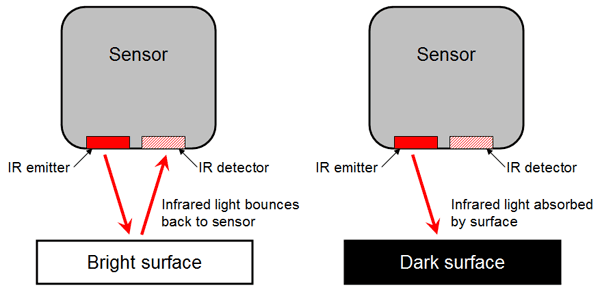
\includegraphics[width=\textwidth]{ir_line.png}
				\caption{Detecting line using IR sensor}
				\label{fig:detect_line_ir}
		\end{figure}
		
		\paragraph{Detecting line using LDR}
		To detect line using LDR same procedure from IR can be used. Since reflected line intensity depends on the reflecting surface. If the color of the surface is white, maximum light is reflected. If it is black then minimum light is reflected. Reflected light has different intensity based on the color of the surface it is being reflected from. So, nearest colors can be differentiated using LDR sensors. 
		
		\begin{figure}[!h]
			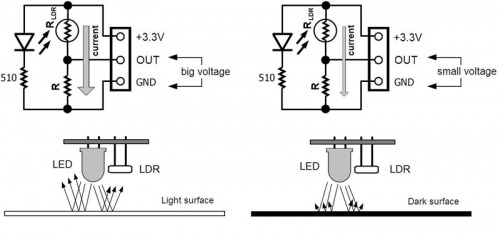
\includegraphics[width=\textwidth]{ldr_line.jpg}
			\caption{Detecting line using LDR sensor}
			\label{fig:detect_line_ldr}
		\end{figure}
		
		%Algorithm code
		
		\subsection{Algorithm for detecting line}
		\begin{algorithm}
		\caption{Line Detecting Algorithm}\label{alg:linetracker}
		\begin{algorithmic}[1]
		\Procedure{detectLine}{\textit{irPin}}
		
		\State $irPin \gets \text{ir receiver pin}$
		\State $irReading \gets \text {analog reading from ir receiver} $
		\State $threshold \gets \text {threshold value for differentiate betweeen white and black line} $
		\State $irDigitalReading \gets \text {converts analog into binary format} $
		
		\State $ irReading \gets \text{reading from irPin}$		
		\If {$irReading > \textit{threshold}$}
		\State $irDigitalReading \gets 1$
		\Else 
		\State $irDigitalReading \gets 0$
		\EndIf
		\EndProcedure
		\end{algorithmic}
		\end{algorithm}
	
	\subsection{Getting current position of the robot using IR / LDR Array}
	Current position of a robot on a line can be extracted by using IR array consisting of two or more than two IR/LDR sensors. Suppose, a robot has an IR array of 5 IR sensors. The spacing between two IR sensor is \textbf{1cm}, and the width of the line is \textbf{1.5cm}. At any time, when the robot is on the line, two values will differ from other three values meaning robot is facing straight, leaning left or leaning right. Depending on the position of the robot on the line, speed of motors can be varied to keep it on the line. This process is completely experimental and varies with the body, circuitry, battery rating, motor rating and mostly other things. The position value can be returned either in binary form such as \textbf{01100} using \ref{alg:linetracker} or in weighted value such as \textbf{2500} from \ref{alg:calculate_position}.
	
	
	\subsubsection{Algorithm for weighted positional value}
	\begin{algorithm}[H]
			\caption{Position calculating algorithm}\label{alg:calculate_position}
			\begin{algorithmic}[1]
			\Procedure{calculatePosition}{\textit{numberOfSensors}}
			\State $numberOfSensors	\gets \text{number of ir/ldr	sensors}$	
			\State  $numberOfActiveSensors \gets 0$
			\State  $digitalReading[numberOfSensors]$ be new array
			\State $weightedValues \gets 0$
			\State $weight \gets 1000$ \Comment{Setting weighted value 1000}
			\State  $position \gets -1$\Comment{Setting current position at -1}
			\For {$index \gets 0$ to $numberOfSensors$}
				\State $digitalReading[index] \gets \Call{detectLine}{index}$
				\If {$digitalReading[index] \gets 1$}
					\State $numberOfActiveSensors \gets numberOfActiveSensors + 1$
				\EndIf
				\State $weightedValues \gets weightedValues + digitalReading[index] * weight$
			\EndFor
			\State $position \gets weightedValues / numberOfActiveSensors$
			\State \textbf{return} $position$
			\EndProcedure		
	\end{algorithmic}
\end{algorithm}
	
	


	\subsection{Conventional line following mechanism}
	
	Conventional line following robots follow lines on a surface based on either predefined conditions or line patterns. Position of the robot can be calculated from  \ref{alg:calculate_position}. If the position of the sensor indicates the robot is being shifted to right from mid point of the line, then the speed of left motor is increased and right motor is decreased and vice versa. If the position of the robot is at middle point then both of the motor will go in the same direction with same speed. The procedure can be viewed from figure \ref{fig:differential_drive_image}.
	
		\begin{figure}[H]
			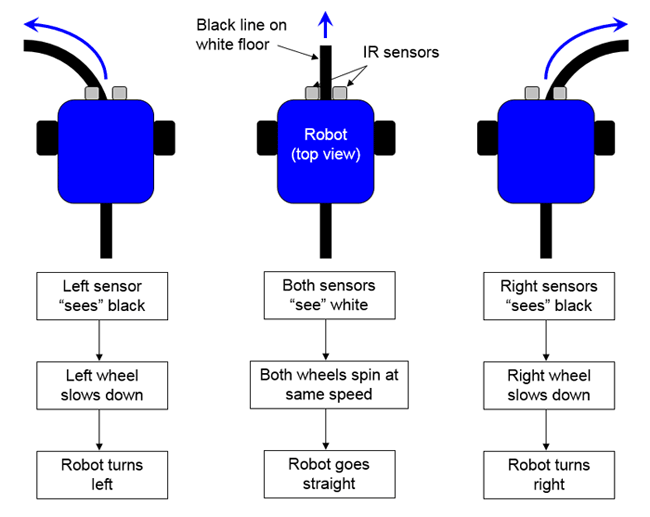
\includegraphics[width=\textwidth]{line-tracking-robot-steering.png}
			\caption{Differential steering drive for following line}
			\label{fig:differential_drive_image}
		\end{figure}
		
	
	\subsection{Drawbacks of line following robot based on differential drive system}
	
	Some drawbacks of differential drive system
	
		\begin{enumerate}
		\item It is a static method that can only be used on a specific robot for which the algorithm was designed
		\item Conditional statements varies with 
			\begin{enumerate}
				\item Weight of the robot
				\item Speed of the robot
				\item Spacing between the IR/LDR sensors of the sensor array
				\item Number of IR/LDR sensors used to make the array
				\item Width of the line to be followed by the robot
			\end{enumerate}
		
		\item This method is not appropriate for driving the robot in right and acute angle turns
		
		
		\end{enumerate}
		
	\section{Machine Learning}
	
	Machine learning is a subfield of computer science that evolved from the study of pattern recognition and computational learning theory in artificial intelligence. In 1959, Arthur Samuel defined machine learning as a ``Field of study that gives computers the ability to learn without being explicitly programmed".
	
		\begin{figure}[H]
			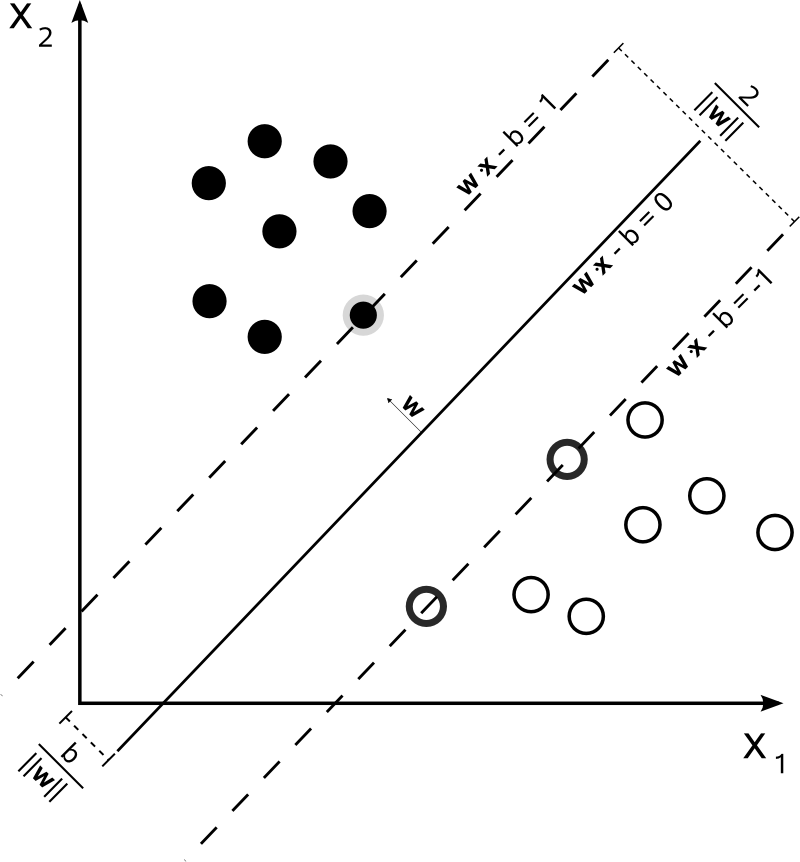
\includegraphics[width=0.5\textwidth, center]{data_classification_svm.png}
			\caption{Support Vector Machine (SVM), an algorithm to classify data}
		\end{figure}
		
		
	\subsection{Model of an Artificial Neuron}
	
	An artificial neuron is a mathematical function conceived as a model of biological neurons. Artificial neurons are the constitutive units in an artificial neural network. Depending on the specific model used they may be called a semi-linear unit, Nv neuron, binary neuron, linear threshold function, or McCulloch–Pitts (MCP) neuron. The artificial neuron receives one or more inputs (representing dendrites) and sums them to produce an output (representing a neuron's axon). Usually the sums of each node are weighted, and the sum is passed through a non-linear function known as an activation function or transfer function. The transfer functions usually have a sigmoid shape, but they may also take the form of other non-linear functions, piecewise linear functions, or step functions. They are also often monotonically increasing, continuous, differentiable and bounded.
	
	\subsubsection{Basic structure}
	
	For a given artificial neuron, let there be $m + 1$ inputs with signals $x_{0}$ through $x_{m}$ and weights $w_{0}$ through $w_{m}$. Usually, the $x_{0}$ input is assigned the value $+1$, which makes it a bias input with $w_{k0} = b_{k}$. This leaves only $m$ actual inputs to the neuron: from $x_{1}$ to $x_{m}$.

	The output of the $k_{th}$ neuron is:	
	\begin{equation}
		y_{k} = \phi \left( \sum_{j = 0}^{m}w_{kj}x_{j} \right)
	\end{equation}
	
	Where $\phi$ (phi) is the transfer function.
	
	\begin{figure} [H]
		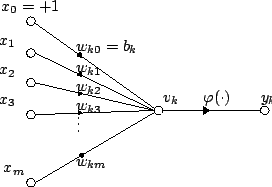
\includegraphics[scale = 0.9, center]{Artificial_neuron.png}
		\caption{Representation of an artificial neuron.}
	\end{figure}
	
	The output is analogous to the axon of a biological neuron, and its value propagates to the input of the next layer, through a synapse. It may also exit the system, possibly as part of an output vector.

It has no learning process as such. Its transfer function weights are calculated and threshold value are predetermined.


	\subsubsection{Comparison to biological neurons}
	
	Artificial neurons are designed to mimic aspects of their biological counterparts.
	
	\begin{enumerate}
		\item \textbf{Dendrites-} In a biological neuron, the dendrites act as the input vector. These dendrites allow the cell to receive signals from a large $(>1000)$ number of neighboring neurons. As in the above mathematical treatment, each dendrite is able to perform "multiplication" by that dendrite's "weight value." The multiplication is accomplished by increasing or decreasing the ratio of synaptic neurotransmitters to signal chemicals introduced into the dendrite in response to the synaptic neurotransmitter. A negative multiplication effect can be achieved by transmitting signal inhibitors (i.e. oppositely charged ions) along the dendrite in response to the reception of synaptic neurotransmitters.
		
		\item \textbf{Soma-}  In a biological neuron, the soma acts as the summation function, seen in the above mathematical description. As positive and negative signals (exciting and inhibiting, respectively) arrive in the soma from the dendrites, the positive and negative ions are effectively added in summation, by simple virtue of being mixed together in the solution inside the cell's body.
		
		\item \textbf{Axon-} The axon gets its signal from the summation behavior which occurs inside the soma. The opening to the axon essentially samples the electrical potential of the solution inside the soma. Once the soma reaches a certain potential, the axon will transmit an all-in signal pulse down its length. In this regard, the axon behaves as the ability for us to connect our artificial neuron to other artificial neurons.
		
	\end{enumerate}
	
	
	\subsubsection{Types of transfer functions}
	
	The transfer function of a neuron is chosen to have a number of properties which either enhance or simplify the network containing the neuron. Crucially, for instance, any multilayer perceptron using a linear transfer function has an equivalent single-layer network; a non-linear function is therefore necessary to gain the advantages of a multi-layer network.

Below, $u$ refers in all cases to the weighted sum of all the inputs to the neuron, i.e. for $n$ inputs,

	\begin{equation}
		u = \sum_{i=1}^n w_{i}x_{i}
	\end{equation}
	
	where $w$ is a vector of \textit{synaptic weights} and \textbf{x} is a vector of inputs.
	
	\paragraph{Step Function}
	
	The output y of this transfer function is binary, depending on whether the input meets a specified threshold, $\theta$. The "signal" is sent, i.e. the output is set to one, if the activation meets the threshold.
	
	\[ y =
		\begin{cases}
		1 & \quad \text{if } u \geq \theta \\
		0 & \quad \text{if } u < \theta \\
		\end{cases}
	\]
	
	
	
	\paragraph{Linear combination}
	In this case, the output unit is simply the weighted sum of its inputs plus a bias term. A number of such linear neurons perform a linear transformation of the input vector. This is usually more useful in the first layers of a network. A number of analysis tools exist based on linear models, such as harmonic analysis, and they can all be used in neural networks with this linear neuron. The bias term allows us to make affine transformations to the data.
	
	\paragraph{Sigmoid}
	A fairly simple non-linear function, a sigmoid function such as the logistic function also has an easily calculated derivative, which can be important when calculating the weight updates in the network. It thus makes the network more easily manipulable mathematically, and was attractive to early computer scientists who needed to minimize the computational load of their simulations.  \textbf{It is commonly seen in multilayer perceptrons using a backpropagation algorithm.}
	

	
	
	\subsection{Artificial Neural Network}
	In machine learning and cognitive science, artificial neural networks (ANNs) are a family of models inspired by biological neural networks (the central nervous systems of animals, in particular the brain) and are used to estimate or approximate functions that can depend on a large number of inputs and are generally unknown. Artificial neural networks are generally presented as systems of interconnected "neurons" which exchange messages between each other. The connections have numeric weights that can be tuned based on experience, making neural nets adaptive to inputs and capable of learning.

For example, a neural network for handwriting recognition is defined by a set of input neurons which may be activated by the pixels of an input image. After being weighted and transformed by a function (determined by the network's designer), the activations of these neurons are then passed on to other neurons. This process is repeated until finally, an output neuron is activated. This determines which character was read.

Like other machine learning methods – systems that learn from data – neural networks have been used to solve a wide variety of tasks that are hard to solve using ordinary rule-based programming, including computer vision and speech recognition.

A basic model of neural network is displayed in figure \ref{fig:neural_net_model}.

		\begin{figure}[H]
			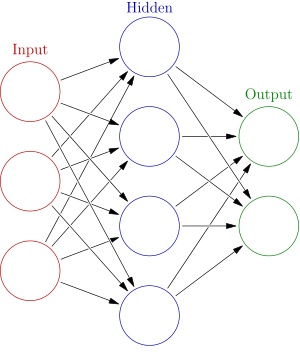
\includegraphics[width=.4\textwidth, center]{neural_net_example.png}
			\caption{Basic model of artificial neural networks}
			\label{fig:neural_net_model}
		\end{figure}
	
	\subsection{Feedforward Neural Network}
	
	A feedforward neural network is an artificial neural network where connections between the units do not form a cycle. This is different from recurrent neural networks.

The feedforward neural network was the first and simplest type of artificial neural network devised. In this network, the information moves in only one direction, forward, from the input nodes, through the hidden nodes (if any) and to the output nodes. There are no cycles or loops in the network.

		\begin{figure}[H]
			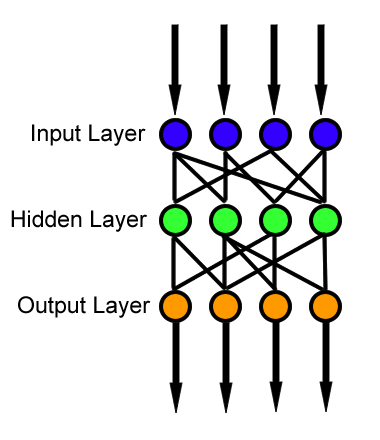
\includegraphics[width=0.4\textwidth, center]{Feed_forward_neural_net.png}
			\caption{A simple Feedforward neural network.}
		\end{figure}
		
		
		\subsubsection{Multi-layer perceptron}
		This class of networks consists of multiple layers of computational units, usually interconnected in a feed-forward way. Each neuron in one layer has directed connections to the neurons of the subsequent layer. In many applications the units of these networks apply a sigmoid function as an activation function.

The universal approximation theorem for neural networks states that every continuous function that maps intervals of real numbers to some output interval of real numbers can be approximated arbitrarily closely by a multi-layer perceptron with just one hidden layer. This result holds for a wide range of activation functions, e.g. for the sigmoidal functions.

		\begin{figure}[H]
			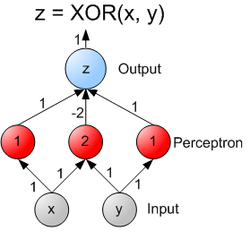
\includegraphics[width=0.4\textwidth, center]{XOR_perceptron_net.png}
			\caption{A multi-layer perceptron network learning XOR}
		\end{figure}
		
		
	\subsubsection{Backpropagation}
	
	Backpropagation, an abbreviation for "backward propagation of errors", is a common method of training artificial neural networks used in conjunction with an optimization method such as gradient descent. The method calculates the gradient of a loss function with respect to all the weights in the network. The gradient is fed to the optimization method which in turn uses it to update the weights, in an attempt to minimize the loss function.
	
	\subsubsection{Gradient descent}
	Gradient descent is a first-order optimization algorithm. To find a local minimum of a function using gradient descent, one takes steps proportional to the negative of the gradient (or of the approximate gradient) of the function at the current point.


	\section{Importance of the project}
	
	Robotics technology is emerging at a rapid pace, offering new possibilities for automating tasks in many challenging applications, especially in autonomous self driving vehicles. A lot of parameters and conditions and other necessary things are needed to be considered to build a complete autonomous self driving vehicles, yet making the vehicle to learn to follow the line of the path is one of the basic building blocks to build a complete autonomous self driving vehicles. The main objective of the project is to train a network and apply it on a autonomous line following prototype which can navigate autonomously at any line consisting of any width. 
	
	Parameters of vehicles can be different from each other but the training techniques to follow a line on a surface will be the same for all of the test objects. So it is more convenient to train the network and set the weight than defining all the conditions to follow line.
	
	
	\section{Prototype construction}
	
	List and description of the items and electronic modules used in this project. 
	
	\subsection{Arduino Nano}
	
	The Arduino Nano is a small, complete, and breadboard-friendly board based on the ATmega328 (Arduino Nano 3.x) or ATmega168 (Arduino Nano 2.x). It has more or less the same functionality of the Arduino Duemilanove, but in a different package. It lacks only a DC power jack, and works with a Mini-B USB cable instead of a standard one. The Nano was designed and is being produced by Gravitech.
	
			\begin{figure}[H]
	\centering
	\begin{minipage}[b]{0.45\linewidth}
		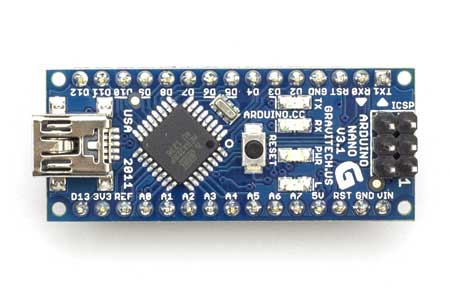
\includegraphics[width=\textwidth, scale=0.5]{ArduinoNanoFront_3_sm.jpg}
		\caption{Arduino Nano Front View}	
	\end{minipage}
	\quad
	\begin{minipage}[b]{0.45\linewidth}
		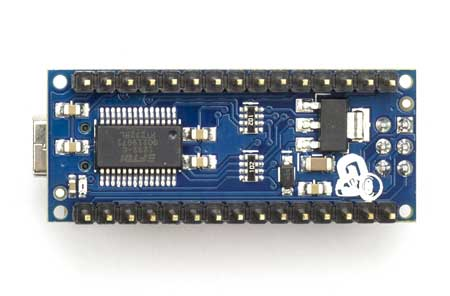
\includegraphics[width=\textwidth, scale=0.5]{ArduinoNanoBack_3_sm.jpg}
		\caption{Arduino Nano Back View}
	
	\end{minipage}
	\end{figure}
	
	

	\subsubsection{Technical Specifications}
	
	\begin{tabular}{| p{5cm} | p{12cm} |}

	\hline
	Microcontroller & Atmel ATmega168 or ATmega328 \\ \hline
	Operating Voltage (logic level) & 5 V \\ \hline
	Input Voltage (recommended) &	7-12 V \\ \hline
	Input Voltage (limits)	& 6-20 V \\ \hline
Digital I/O Pins &	14 (of which 6 provide PWM output)\\ \hline
Analog Input Pins &	8 \\ \hline
DC Current per I/O Pin & 40 mA \\ \hline
Flash Memory &	16 KB (ATmega168) or 32 KB (ATmega328) of which 2 KB used by bootloader \\ \hline
SRAM &	1 KB (ATmega168) or 2 KB (ATmega328)\\ \hline
EEPROM	& 512 bytes (ATmega168) or 1 KB (ATmega328)\\ \hline
Clock Speed &	16 MHz \\ \hline
Dimensions &	0.73" x 1.70" \\ \hline
Length &	45 mm\\ \hline
Width &	18 mm\\ \hline
Weight	& 5 g\\ \hline
	
	\end{tabular}

	
	\subsection{QTR-8A Reflectance Sensor Array}
	
	This sensor module has 8 IR LED/phototransistor pairs mounted on a 0.375" pitch. Pairs of LEDs are arranged in series to halve current consumption, and a MOSFET allows the LEDs to be turned off for additional sensing or power-savings options. Each sensor provides a separate analog voltage output.
	
	\begin{figure}[H]
		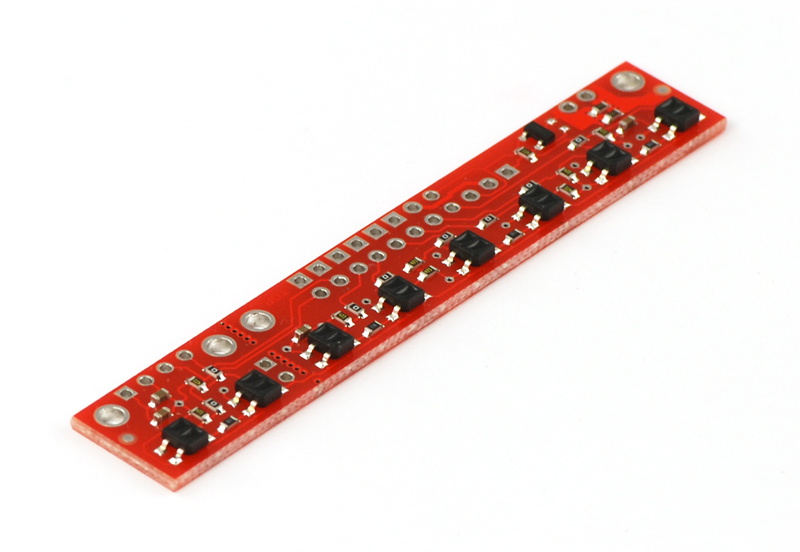
\includegraphics[scale=.28, center]{qtr.jpg}
		\caption{Pololu QTR-8A Reflectance Sensor Array}
	\end{figure}
	
	\subsection{L298N Motor Driver}
	
	To drive two motors, L298N stepper motor driver breakout was used.
	
	\begin{figure}[H]
		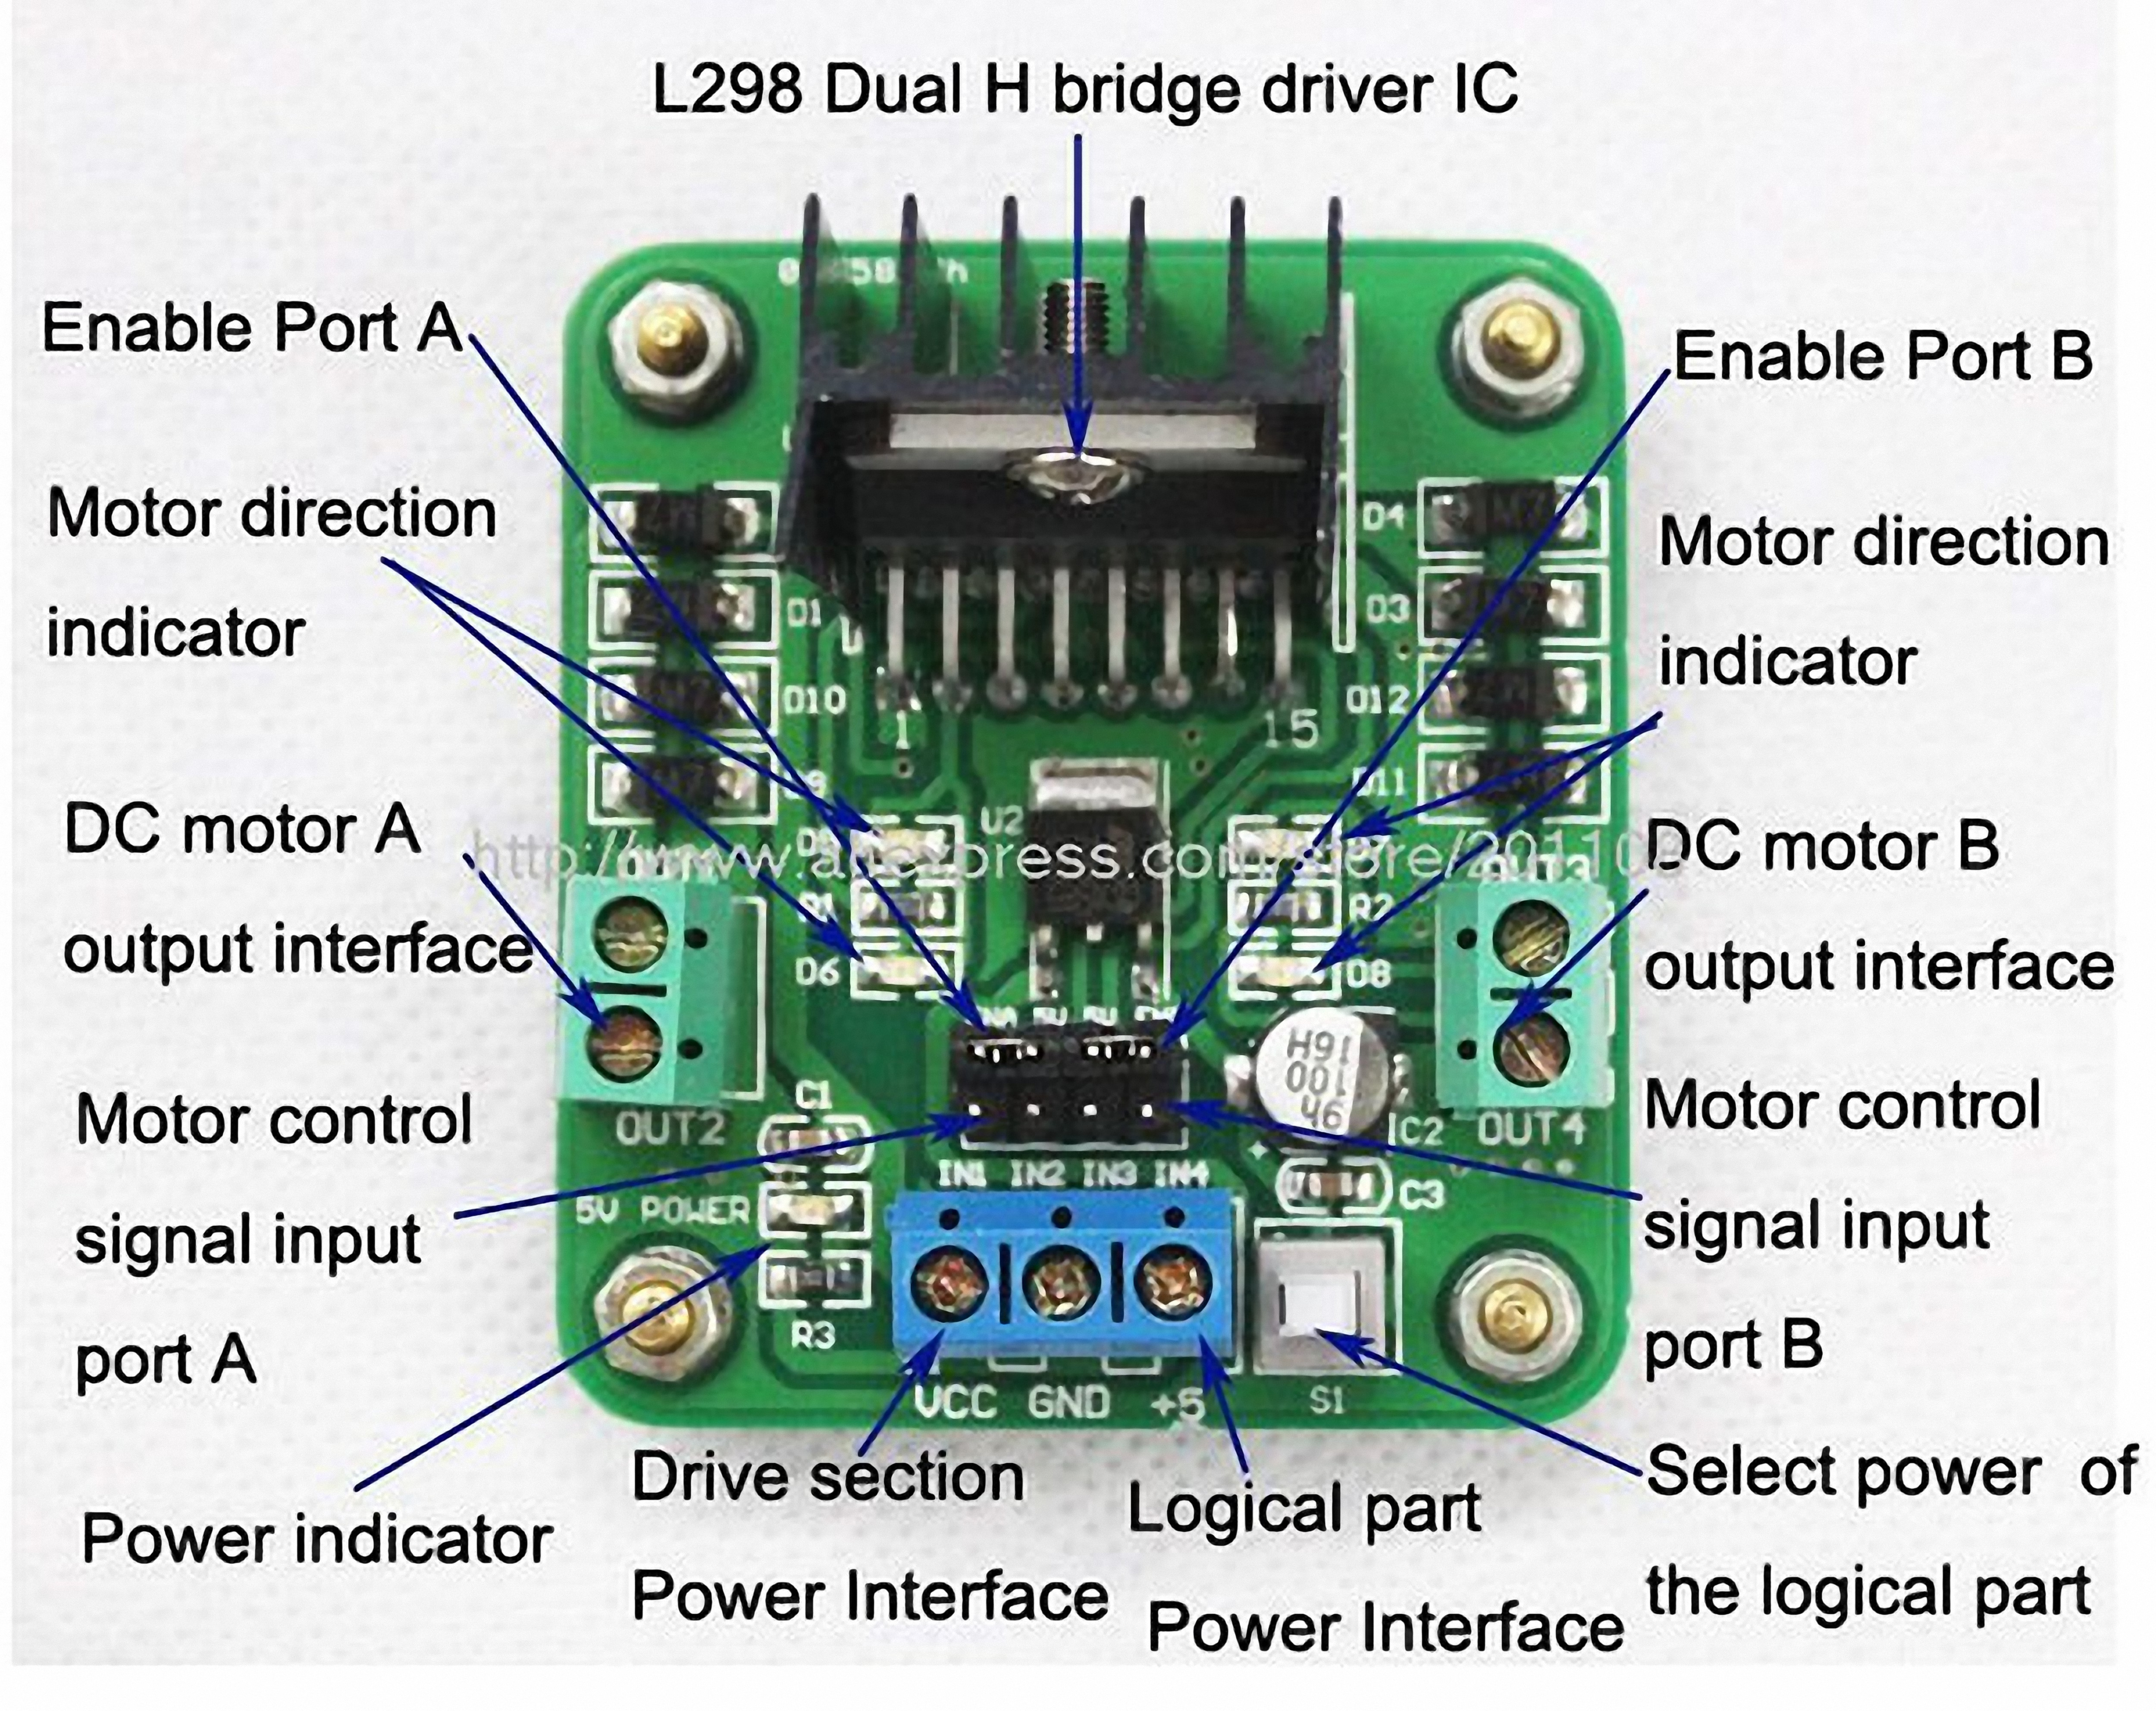
\includegraphics[scale=0.5,center]{l298n.jpg}
		\caption{L298N DC Motor Driver}
	\end{figure}
	
	\subsection{Lithium-Polymer Battery}
	
	A 3 cell Li-Po battery was used with 800mAh capacity.
	
	\begin{figure}[H]
		
\includegraphics[center]{lipo.jpg}
		\caption{3 Cell 800mAh Li-Po Battery}
	\end{figure}
	
	
		\subsection{Bluetooth Module}
	
	HC-05 module is an easy to use Bluetooth SPP (Serial Port Protocol) module, designed for transparent wireless serial connection setup. Serial port Bluetooth module is fully qualified Bluetooth V2.0+EDR (Enhanced Data Rate) 3Mbps Modulation with complete 2.4GHz radio transceiver and baseband. It uses CSR Bluecore 04-External single chip Bluetooth system with CMOS technology and with AFH(Adaptive Frequency Hopping Feature). It has the footprint as small as  $ {12.7mm \times 27mm}$.
	
	\paragraph{Hardware Features}

	\begin{enumerate}

	\item Typical $-80dBm$ sensitivity
	\item Up to $+4dBm$ RF transmit power
	\item Low Power 1.8V Operation
	\item UART interface with programmable baud rate
	\item With edge connector
	\end{enumerate}
	
	\begin{figure}[H]
		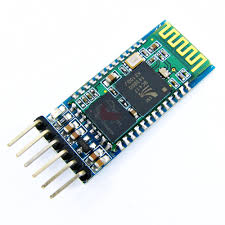
\includegraphics[center]{hc05.jpg}
		\caption{HC-05 Bluetooth Module}
	\end{figure}

	\subsection{Breadboard}
	
	For completing the circuit of the prototype I used small breadboard to connect the wires. 
	
	\begin{figure}[H]
		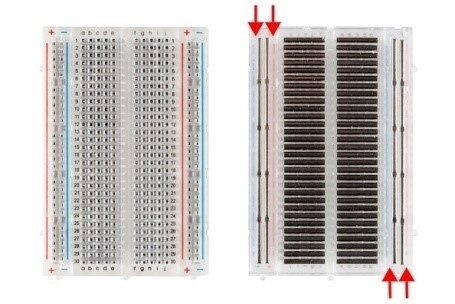
\includegraphics[center]{breadboard.jpg}
		\caption{Half size breadboard (clear)}
	\end{figure}
	
	\subsection{Premium Jumper Wire}
	
	Male to male and male to female jumper connectors to connect the components together.
	
	\begin{figure}[H]
		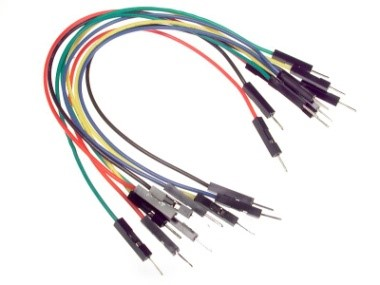
\includegraphics[center]{jumper.jpg}
		\caption{Connecting wires}
	\end{figure}


	\section{Sensor positioning of the prototype}
	
	\section{Circuit diagram}
	
		\begin{figure}[H]
			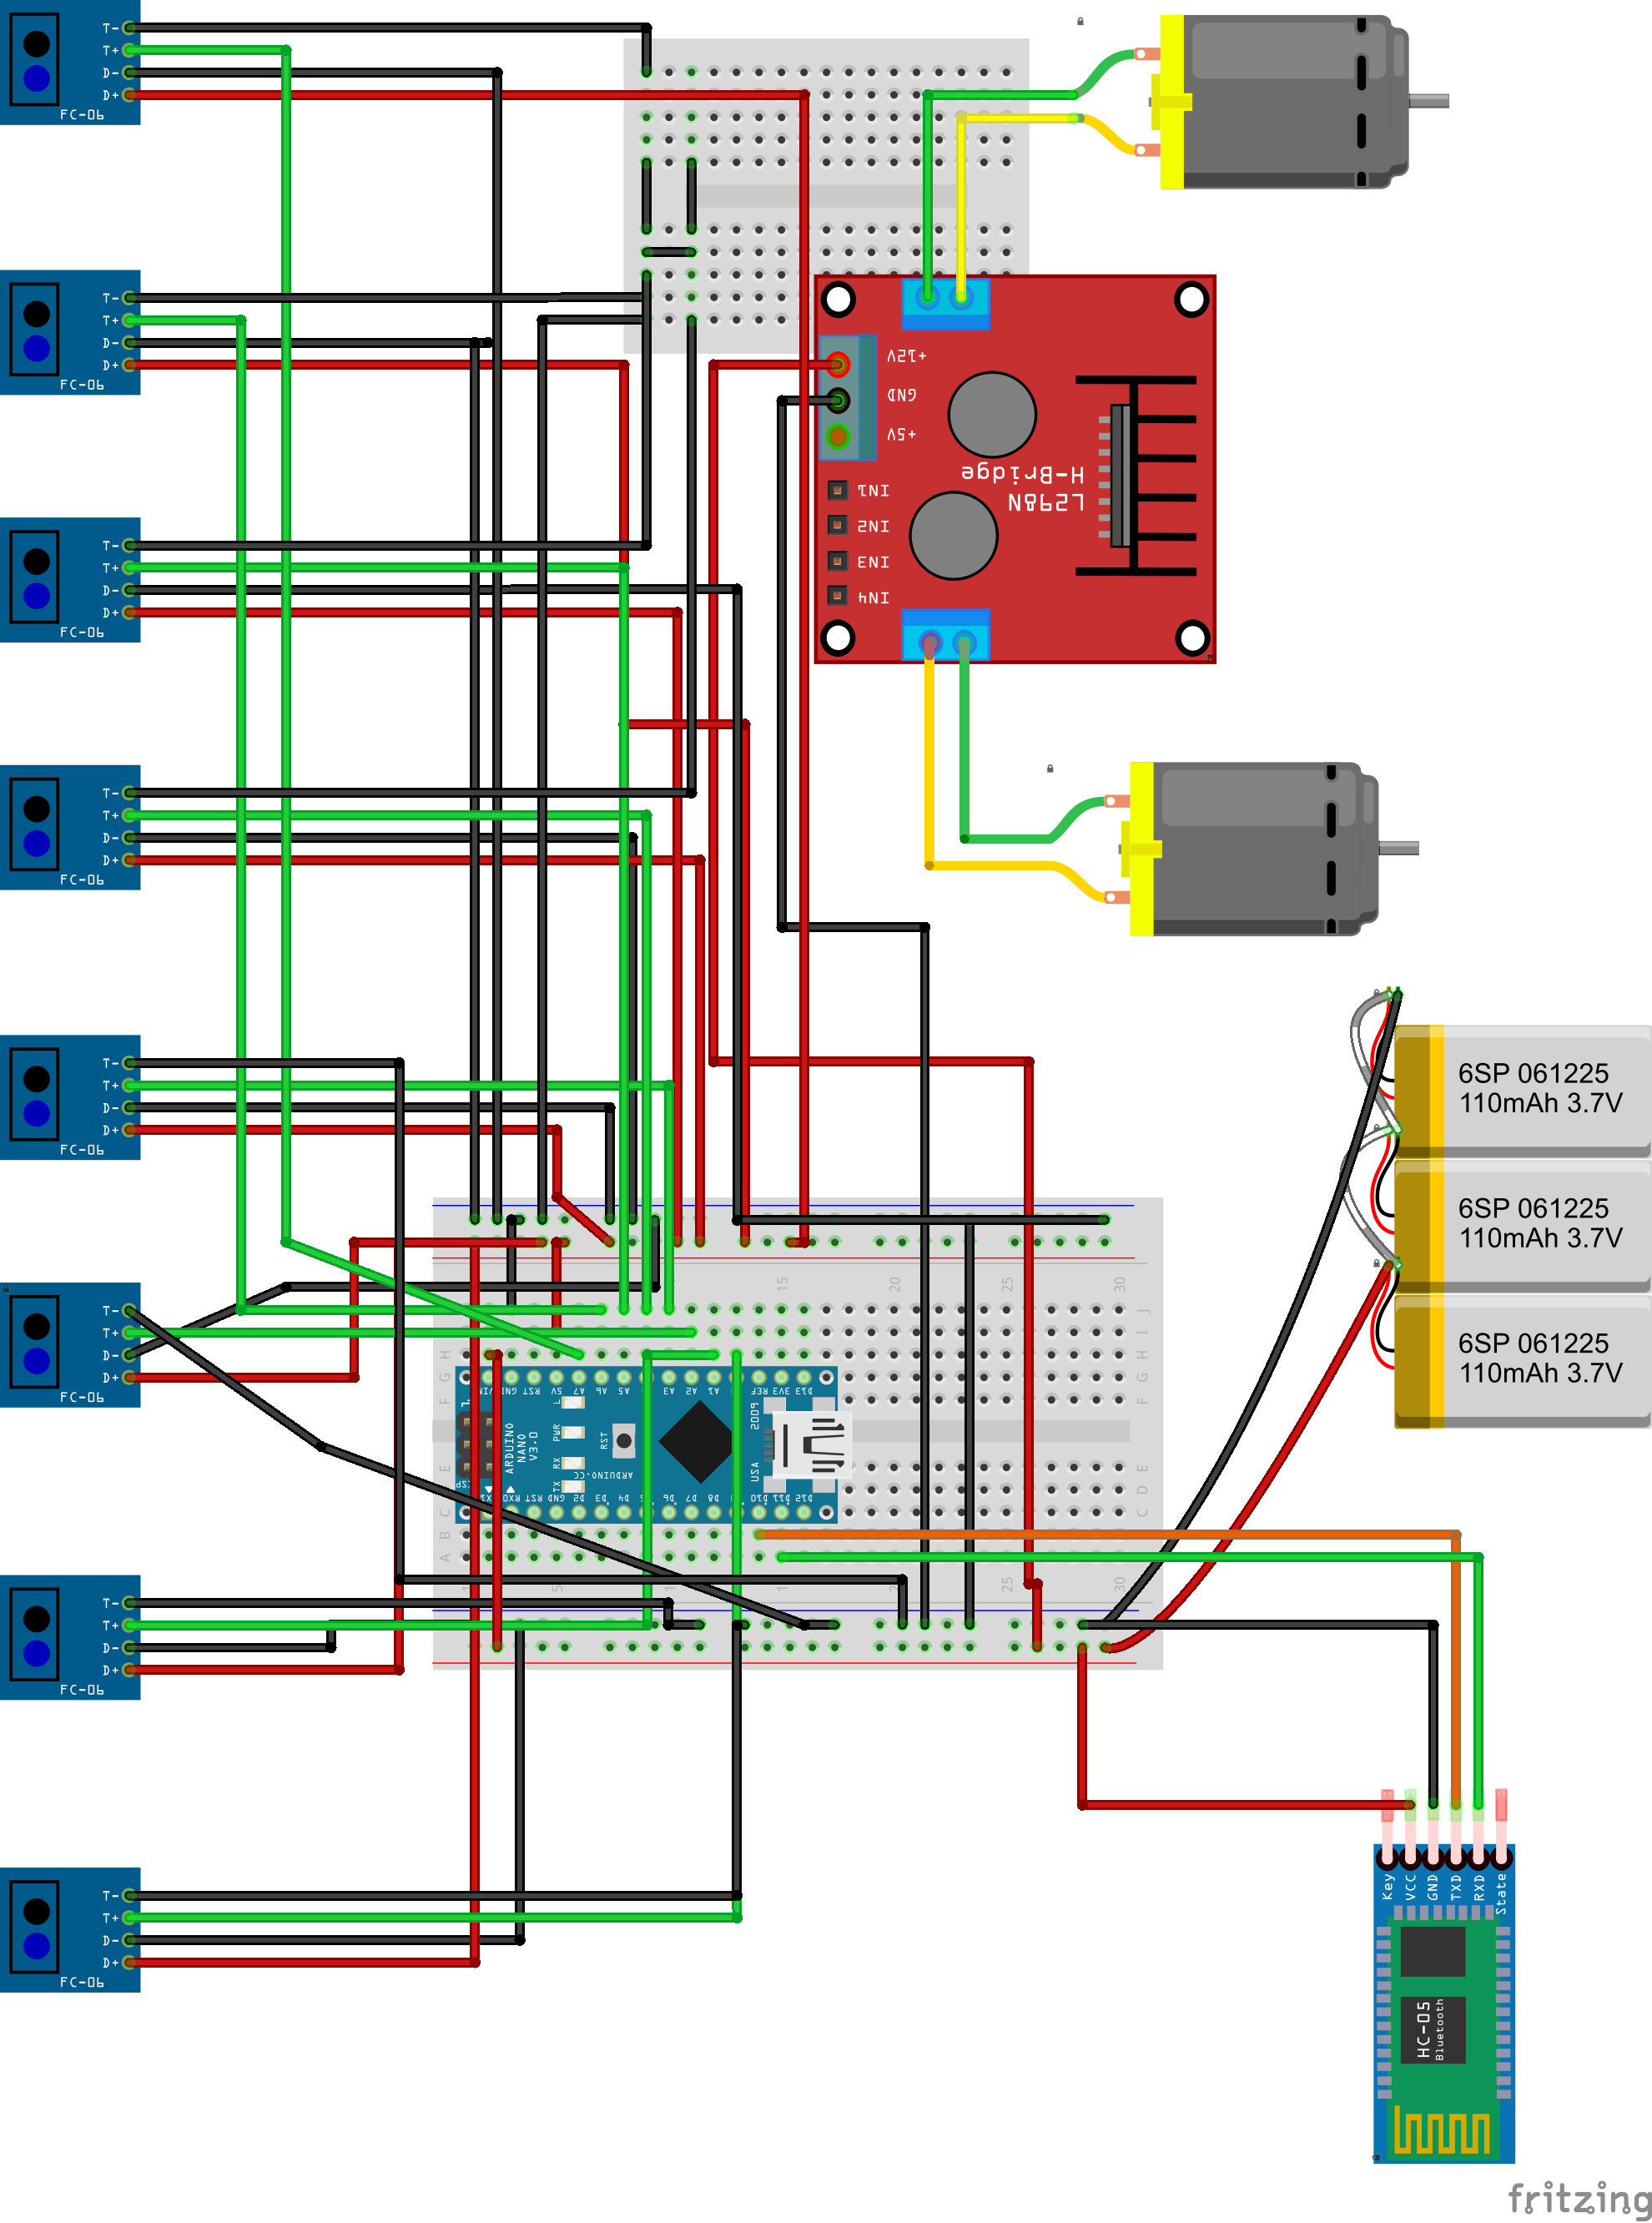
\includegraphics[left, scale = 0.8]{ckt_diagram.png}
			\caption{Circuit diagram of the robotic platform.}
		\end{figure}
	
	
	\section{Data collection process}
	
	\subsection{Processing code for driving and collecting data wirelessly}
	
		\begin{verbatim}
		
				import processing.serial.*;
int value = 0;
int width = 50;
int height = 50;
final int baud = 9600;

Serial arduino;

void setup(){
  String arduinoPort = "COM12";
  println(Serial.list());
  arduino = new Serial(this, arduinoPort, baud);
}

char old_key = '0';
char new_key = '1';

//Checking if any key was pressed, initializing with a 'false'
boolean wasPressed = false;

void serialEvent(Serial port){
  String inByte = port.readStringUntil('\n');
  if (inByte != null) println(inByte);
}

void draw(){
  if (keyPressed == true){
    new_key = key;
    if (new_key != old_key) {
      arduino.write(key);
    }
    wasPressed = true;
  } else {
    if (wasPressed == true){
      new_key = 'z';
      arduino.write('z');
      wasPressed = false;
    }
  }
  old_key = new_key;
}
		
		\end{verbatim}

	\subsection{Arduino code for the robotic prototype}
	
	\subsubsection{LineFollower.h}
	
	\begin{verbatim}
#ifndef LINE_FOLLOWER_H_
#define LINE_FOLLOWER_H_
#include <Arduino.h>
#include <StandardCplusplus.h>
#include <vector>
#include <serstream>
#include <iterator>
#include <SoftwareSerial.h>

using namespace std;

//If inverse logic is defined
#if defined(INVERSE_LOGIC)
	#define INSIDE_LINE 0
	#define OUTSIDE_LINE 1
#else
	#define INSIDE_LINE 1
	#define OUTSIDE_LINE 0
#endif

///define front and back pin
#define FRONT_PIN 0
#define BACK_PIN 1

#define BAUD 9600
#define DEFAULT_SPEED 150
#define MULTIPLIER 1000

#define RX 10
#define TX 11

//Delay macro
#define SHORT_DELAY 100
#define LONG_DELAY 500

//Threshold
#define THRESHOLD 500

//add and subtract from or to this speed
#define spd 85
#define speed_factor 10
#define spd_factor 4
#define add_speed 60

//define input and output macro
#define input(pin) pinMode(pin, INPUT)
#define output(pin) pinMode(pin, OUTPUT)

//Define high low and pwm macro
#define pwm(pin, value) analogWrite(pin, value)
#define on(pin) digitalWrite(pin, HIGH)
#define off(pin) digitalWrite(pin, LOW)

#define short_delay delay(SHORT_DELAY)
#define long_delay delay(LONG_DELAY)

typedef unsigned int u_int;

class LineFollower
{
private:

  u_int leftMotorPin[2];
  u_int rightMotorPin[2];
  u_int defaultSpeed;
  vector <u_int> sensors;
  u_int leftSpeed;
  u_int rightSpeed;
  char command;
  u_int activeSensors;
public:
	//Digital and analog reading array
	vector <u_int> digitalReading;
	vector <u_int> analogReading;

    //Constructors
    LineFollower(void) :
	defaultSpeed(DEFAULT_SPEED),
	activeSensors(0)
	{
		leftSpeed = DEFAULT_SPEED;
		rightSpeed = DEFAULT_SPEED;
	};

    LineFollower(u_int *lm, u_int *rm, vector <u_int> &s);

    //Initializer
    void serial_init(u_int b);
    void init(void);
	void sensors_init(void);
	void sensors_init(vector <u_int> &s);
	void set_sensors_pins(vector <u_int> s);

    //Motor config functions
    void set_motors_pins(u_int *lm, u_int *rm);
    void set_motors(int lspeed, int rspeed);
    void motors_init(void);
	void stop(void);
	void set_speed(u_int dSpeed);

	//Extra motor controls
	void forward(u_int lspeed, u_int rspeed);
	void backward(u_int lspeed, u_int rspeed);
	void left(u_int rspeed);
	void right(u_int lspeed);
	void anticlockwise(u_int lspeed, u_int rspeed);
	void clockwise(u_int lspeed, u_int rspeed);

	//Bluetooth control
	void wireless_control(void);
	void wireless_control(bool debug_mode);

	//Debugging sensors
	void debug(void);
	void wireless_debug(void);

	//Line Following control
	void read_sensors(void);
	int read_line(void);
	void clear_reading(void);
	void conditional_drive(void);
};

extern LineFollower LineFollowingRobot;
extern SoftwareSerial Bluetooth;
#endif
	\end{verbatim}
	
	
	\subsubsection{LineFollower.cpp}
	
	\begin{spverbatim}
#include <LineFollower.h>

//Objects created for line following robot and bluetooth
LineFollower LineFollowingRobot;
SoftwareSerial Bluetooth(RX, TX);

namespace std
{
  ohserialstream cout(Serial);
}

using namespace std;

//Initialize everything
void LineFollower::init(void)
{
  motors_init();
  sensors_init();
  serial_init(BAUD);
  defaultSpeed = DEFAULT_SPEED;
  input(0);
  input(7);
}

//========== MOTOR SECTION ==============
//Initialize motors
void LineFollower::motors_init(void)
{
  for (u_int i = 0; i < 2; i++)
  {
    pinMode(leftMotorPin[i], OUTPUT);
    pinMode(rightMotorPin[i], OUTPUT);
  }
}

//Run the motors
void LineFollower::set_motors(int lspeed, int rspeed)
{
  //Forward || Left || Right
  if (lspeed >= 0 && rspeed >= 0)
  {
    leftSpeed = lspeed;
    rightSpeed = rspeed;
    pwm(leftMotorPin[FRONT_PIN], leftSpeed);
    pwm(rightMotorPin[FRONT_PIN], rightSpeed);
    off(leftMotorPin[BACK_PIN]);
    off(rightMotorPin[BACK_PIN]);
  }
  //Right || Clockwise
  else if (lspeed >= 0 && rspeed < 0)
  {
    leftSpeed = lspeed;
    rightSpeed = -rspeed;
    pwm(leftMotorPin[FRONT_PIN], leftSpeed);
    off(leftMotorPin[BACK_PIN]);
    pwm(rightMotorPin[BACK_PIN], rightSpeed);
    off(rightMotorPin[FRONT_PIN]);
  }
  //Left || Anticlockwise
  else if (lspeed < 0 && rspeed >= 0)
  {
    leftSpeed = -lspeed;
    rightSpeed = rspeed;
    pwm(rightMotorPin[FRONT_PIN], rightSpeed);
    off(rightMotorPin[BACK_PIN]);
    pwm(leftMotorPin[BACK_PIN], leftSpeed);
    off(leftMotorPin[FRONT_PIN]);
  }
  //Backward
  else if (lspeed < 0 && rspeed < 0)
  {
    leftSpeed = -lspeed;
    rightSpeed = -rspeed;
    pwm(leftMotorPin[BACK_PIN], leftSpeed);
    pwm(rightMotorPin[BACK_PIN], rightSpeed);
    off(leftMotorPin[FRONT_PIN]);
    off(rightMotorPin[FRONT_PIN]);
  }
  //Stop
  else stop();
}

//Extra motor controls
void LineFollower::forward(u_int lspeed, u_int rspeed)
{
  leftSpeed = lspeed;
  rightSpeed = rspeed;
  pwm(leftMotorPin[FRONT_PIN], leftSpeed);
  pwm(rightMotorPin[FRONT_PIN], rightSpeed);
  off(leftMotorPin[BACK_PIN]);
  off(rightMotorPin[BACK_PIN]);
}

void LineFollower::backward(u_int lspeed, u_int rspeed)
{
  leftSpeed = lspeed;
  rightSpeed = rspeed;
  pwm(leftMotorPin[BACK_PIN], leftSpeed);
  pwm(rightMotorPin[BACK_PIN], rightSpeed);
  off(leftMotorPin[FRONT_PIN]);
  off(rightMotorPin[FRONT_PIN]);
}

void LineFollower::left(u_int rspeed)
{
  rightSpeed = rspeed;
  off(leftMotorPin[BACK_PIN]);
  off(leftMotorPin[FRONT_PIN]);
  pwm(rightMotorPin[FRONT_PIN], rightSpeed);
  off(rightMotorPin[BACK_PIN]);
}

void LineFollower::right(u_int lspeed)
{
  leftSpeed = lspeed;
  off(rightMotorPin[FRONT_PIN]);
  off(rightMotorPin[BACK_PIN]);
  pwm(leftMotorPin[FRONT_PIN], leftSpeed);
  off(leftMotorPin[BACK_PIN]);
}

void LineFollower::clockwise(u_int lspeed, u_int rspeed)
{
  leftSpeed = lspeed;
  rightSpeed = rspeed;
  pwm(leftMotorPin[FRONT_PIN], leftSpeed);
  off(leftMotorPin[BACK_PIN]);
  pwm(rightMotorPin[BACK_PIN], rightSpeed);
  off(rightMotorPin[FRONT_PIN]);
}

void LineFollower::anticlockwise(u_int lspeed, u_int rspeed)
{
  leftSpeed = lspeed;
  rightSpeed = rspeed;
  pwm(leftMotorPin[FRONT_PIN], leftSpeed);
  off(leftMotorPin[BACK_PIN]);
  pwm(rightMotorPin[BACK_PIN], rightSpeed);
  off(rightMotorPin[FRONT_PIN]);
}

//Set the motor pins
void LineFollower::set_motors_pins(u_int *lm, u_int *rm)
{
  for (u_int i = 0; i < 2; i++){
    leftMotorPin[i] = lm[i];
    rightMotorPin[i] = rm[i];
  }
}

void LineFollower::stop(void)
{
  for (u_int i = 0; i < 2; i++){
    off(leftMotorPin[i]);
    off(rightMotorPin[i]);
  }
}

void LineFollower::set_speed(u_int dSpeed)
{
  defaultSpeed = dSpeed;
}

/*========= SENSOR ==============*/
//Initialize sensors
void LineFollower::sensors_init(void)
{
  for (u_int i = 0; i < sensors.size(); i++)
    pinMode(sensors[i], INPUT);
}

void LineFollower::sensors_init(vector <u_int> &s)
{
  sensors = s;
  for (u_int i = 0; i < sensors.size(); i++) pinMode(sensors[i], INPUT);
}

void LineFollower::set_sensors_pins(vector <u_int> s)
{
  sensors_init(s);
}

/*== DEBUG SECTION*/
//Print sensor value
void LineFollower::debug(void)
{
  long_delay;
  cout << " ======= ANALOG READING ===== " << endl;
  for (u_int i = 0; i < sensors.size(); i++)
  {
    cout << "ir [" << (i + 1) << "] = " << analogRead(sensors[i]) << endl;
    short_delay;
  }
  cout << " ====== ANALOG READING END ======" << endl;
  cout << endl << endl;
  short_delay;
  cout << " ======= DIGITAL READING ======= " << endl;
  read_sensors();
  short_delay;
  for (u_int i = 0; i < sensors.size(); i++)
    cout << digitalReading[i] << " ";
  cout << endl;
  cout << " ======= DIGITAL READING END ==== " << endl;
  cout << endl << endl;
  long_delay;
}

void LineFollower::wireless_debug(void)
{
  long_delay;
  Bluetooth.println("======= ANALOG READING ===== ");
  for (u_int i = 0; i < sensors.size(); i++){
    Bluetooth.println("ir [" + String(i + 1) + "] = " + String(analogRead(sensors[i])));
    short_delay;
  }
  Bluetooth.println("======= ANALOG READING END ===== ");
  Bluetooth.println();
  Bluetooth.println();
  short_delay;

  Bluetooth.println(" ==== DIGITAL READING START === ");
  read_sensors();
  short_delay;
  
  for (u_int i = 0; i < sensors.size(); i++)
    Bluetooth.print(digitalReading[i] + String(" "));
    
  Bluetooth.println();
  Bluetooth.println("====== DIGITAL READING END ======");
  Bluetooth.println();
  Bluetooth.println("Calculated position: " + String(read_line()));
  Bluetooth.println();
  long_delay;
}

// LINE FOLLOWING CONTROL
void LineFollower::read_sensors(void)
{
  digitalReading.clear();
  analogReading.clear();
  activeSensors = 0;
  for (u_int i = 0; i < sensors.size(); i++) {
    u_int reading = analogRead(sensors[i]);
    analogReading.push_back(reading);
    if (reading > THRESHOLD){
      digitalReading.push_back(INSIDE_LINE);
      activeSensors++;
    }
    else
      digitalReading.push_back(OUTSIDE_LINE);
  }
}

void LineFollower::clear_reading(void)
{
  digitalReading.clear();
  analogReading.clear();
}

int LineFollower::read_line(void)
{
  u_int totalWeight = 0;
  read_sensors();
  for (u_int i = 0; i < sensors.size(); i++)
  {
    totalWeight += (i + 1) * digitalReading[i] * MULTIPLIER;
  }
  return (totalWeight / activeSensors);
}

//Driving definition
void LineFollower::conditional_drive(void)
{
  read_line();
  if (digitalReading[3] == 1 || digitalReading[4] == 1)
    forward(defaultSpeed, defaultSpeed);
  else if (digitalReading[2] == 1)
    forward(0, add_speed + speed_factor * 1.5);
  else if (digitalReading[1] == 1)
    forward(0, add_speed + speed_factor * 2.5);
  else if (digitalReading[0] == 1)
    forward(0, add_speed + speed_factor * 3.5);
  else if (digitalReading[5] == 1)
    forward(add_speed + speed_factor * 1.5, 0);
  else if (digitalReading[6] == 1)
    forward(add_speed + speed_factor * 2.5, 0);
  else if (digitalReading[7] == 1)
    forward(add_speed + speed_factor * 3.5, 0);
  else if (digitalReading[0] == 1 && digitalReading[1] == 1)
    forward(0, add_speed + speed_factor * 3);
  else if (digitalReading[6] == 1 && digitalReading[7] == 1)
    forward(add_speed + speed_factor * 3, 0);
  else stop();
}

bool LineFollower::check_left_turn(void)
{
  int leftReading = analogRead(7);
  if (leftReading > THRESHOLD) return true;
  else return false;
}

bool LineFollower::check_right_turn(void)
{
  int rightReading = analogRead(0);
  if (rightReading > THRESHOLD) return true;
  else return false;
}

/*
//  =========== CONSTRUCTOR ==========
*/
//Ctor
LineFollower::LineFollower(u_int *lm, u_int *rm, vector <u_int> &s)
: defaultSpeed(DEFAULT_SPEED),
  activeSensors(0) {
  sensors = s;
  for (u_int i = 0; i < 2; i++)
  {
    leftMotorPin[i] = lm[i];
    rightMotorPin[i] = rm[i];
  }
}

//Initialize serial communication
void LineFollower::serial_init(u_int baud)
{
  Serial.begin(baud);
  Bluetooth.begin(baud);
}

//========== WIRELESS CONTROL ========
void LineFollower::wireless_control(void)
{
  if (Bluetooth.available() > 0) 
  	command = Bluetooth.read();
  switch (command)
  {
    case 'w':
      forward(defaultSpeed, defaultSpeed);
      break;
    case 's':
      backward(defaultSpeed, defaultSpeed);
      break;
    case 'a':
      left(defaultSpeed);
      break;
    case 'd':
      right(defaultSpeed);
      break;
    case 'r':
      wireless_debug();
      break;
    default:
      stop();
      break;
  }
}

void LineFollower::wireless_control(bool debug_mode)
{
  if (!debug_mode) wireless_control();
  else
  {
    if (Bluetooth.available() > 0){
      command = Bluetooth.read();
      Serial.println("I received: " + String(command));
    }
    switch (command){
      Bluetooth.println(command);
      case 'w':
        forward(defaultSpeed, defaultSpeed);
        Bluetooth.println("FORWARD");
        Serial.println("FORWARD");
        break;
      case 's':
        backward(defaultSpeed, defaultSpeed);
        Bluetooth.println("BACKWARD");
        Serial.println("BACKWARD");
        break;
      case 'a':
        left(defaultSpeed);
        Bluetooth.println("LEFT");
        Serial.println("LEFT");
        break;
      case 'd':
        right(defaultSpeed);
        Bluetooth.println("RIGHT");
        Serial.println("RIGHT");
        break;
      case 'r':
        wireless_debug();
        break;
      default:
        Bluetooth.println("STOP");
        Serial.println("STOP");
        stop();
        break;
    }
  }
}

	\end{spverbatim}


\end{document}

	
